% vim: set textwidth=78 autoindent:
%%%%%%%%%%%%%%%%8%%%%%%%%%%%%%%%%%%%%%%%%%%%%%%%%%%%
%
% This is a collection of macros to maintain a uniform style throughout
% the user guide.
% Many of the styles are intended to mimic the appearance of the GUI.
% In general, the objective is to use the non-hover appearance, so a user
% can visually scan the GUI to find something that looks like the instruction
% in the user guide.
% Text styles related to coding are used to indicate different kinds of
% entities, such as classes, methods, etc, and therefore don't correspond to
% any actual appearance.
%
% TEXT STYLES
% These styles change the text appearance but don't add any shadow boxes
% and should be used to refer to non-GUI text (command line, code)
% or non-clickable GUI text (labels).
%
% usertext
% generic style for text that the user should type in from the keyboard
% Note: for user input into a labelled text field in the GUI, see \inputtext
% usage: \usertext{qgis ---help}
\newcommand{\usertext}[1]{\texttt{#1}}
%
% filename
% usage: \filename{lakes.shp}
\newcommand{\filename}[1]{\texttt{#1}}
%
% server
% usage: \server{myhost.de}
\newcommand{\server}[1]{\textit{#1}}
% keystroke
% style for user input by individual keystrokes
% usage: \keystroke{p}, \keystroke{Ctrl+B}
\newcommand{\keystroke}[1]{\cornersize{.6}\ovalbox{\textsf{#1}}}
%
% guilabel
% generic style for text that appears in the GUI
% usage
\newcommand{\guilabel}[1]{\textsf{#1}}
%
% guiheading
% style for section heading that appear in dialog boxes
% such as Vector Layer Properties > metadata
% usage
\newcommand{\guiheading}[1]{\textsf{#1}}
%
% dialog
% usage: \dialog{Layer Properties}
\newcommand{\dialog}[1]{
\fcolorbox[rgb]{0.2,0.2,0.95}[rgb]{0.2,0.2,0.95}{%
\textbf{\textcolor{white}{#1}}}}
%
% Here are some styles for use only when discussing Python coding
% classname
% usage: \classname{NewLayer}
\newcommand{\classname}[1]{\textsf{\textbf{#1}}}
%
% object
% usage
\newcommand{\object}[1]{\textsf{\textit{#1}}}
%
% method
% usage: \method{classFactory}
\newcommand{\method}[1]{\textsf{\textit{#1}}}
%
% fieldname: part of the set intend to be used to describe Python coding.
% So "field" in this case refers to data members of a class or object, not 
% a "field" from a table or database.
% I have commented out this macro, because it wasn't actually used in the 
% creating_applications section.
% For "fields" from a table or database, use one of the following
% 1. When the field name is something a user should type in, use \usertext
% 2. When the field name is something that the user will see in the GUI, but not 
% click on, use \guilabel
% 3. When the field name is something that the user will select from a selection 
% field, use \selectstring. This requires two parameters, one for the 
% label, the other for the selected text.
%\newcommand{\fieldname}[1]{\textsl{#1}}% 

%
% ??? these styles are from Gary: use only in 
%\newcommand{\sqltable}[1]{\textsf{\textbf{#1}}}


% CLICKABLE STYLES
% These styles add a shadow box to indicate the user can click on something
% this command sets the shadow size for the entire document
\setlength{\shadowsize}{2pt}%

% button: for any button that only has text, no icon
% usage: \button{Save as Default}
\newcommand{\button}[1]{%
\raisebox{-6pt}{%
\shadowbox{\guilabel{#1}}
}}
% mainmenuopt: for the top level menus such as File
% usage: \mainmenuopt{Layer}
\newcommand{\mainmenuopt}[1]{%
\raisebox{-6pt}{%
\setlength{\fboxsep}{0pt}%
\shadowbox{\setlength{\fboxsep}{2pt}%
\fcolorbox[gray]{0.9}[gray]{0.9}%
{\guilabel{#1}}%
}}}
% dropmenuopt: for dropdown menu items with no icon
% usage: \mainmenuopt{View} > \dropmenuopt{Toolbar Visibility}
\newcommand{\dropmenuopt}[1]{%
\raisebox{-6pt}{{%
\setlength{\fboxsep}{0pt}%
\shadowbox{\setlength{\fboxsep}{2pt}%
\fcolorbox[rgb]{.95,.95,0.8}[rgb]{.95,.95,0.8}%
{ \guilabel{#1}}}%
}}}
% dropmenucheck: for dropdown menu checkboxes
% usage: \mainmenuopt{View} > \dropmenucheck{Legend}
\newcommand{\dropmenucheck}[1]{%
\raisebox{-6pt}{{%
\setlength{\fboxsep}{0pt}%
\shadowbox{\setlength{\fboxsep}{2pt}%
\fcolorbox[rgb]{.95,.95,0.8}[rgb]{.95,.95,0.8}%
{ $\boxtimes$ \guilabel{#1}}}%
}}}
% dropmenuopttwo: for dropdown menu items with icons
% usage: \mainmenuopt{Layer} > 
% \dropmenuopttwo{mActionAddRasterLayer}{Add a Raster Layer}
\newcommand{\dropmenuopttwo}[2]{%
\raisebox{-6pt}{%
{%
\setlength{\fboxsep}{0pt}%
\shadowbox{\setlength{\fboxsep}{2pt}%
\fcolorbox[rgb]{.95,.95,0.8}[rgb]{.95,.95,0.8}%
{\includegraphics[width=3mm]{#1} \guilabel{#2}}}%
}}}
% tooltip: for the tooltip that appears when hovering on a tool button
% usage
\newcommand{\tooltip}[1]{%
\raisebox{-2pt}{%
\fcolorbox{black}[rgb]{1,1,0.8}{\guilabel{#1}}%
}}
% toolbtntwo: for toolbar items
%usage: \toolbtntwo{mActionAddRasterLayer}{Add a Raster Layer}
%
\newcommand{\toolbtntwo}[2]{%
\raisebox{-6pt}{%
\shadowbox{\includegraphics[width=7mm]{#1}}} %
\tooltip{#2}%
}
%\toolbox
%Used only for menu items (modules) in the GRASS toolbox. 
%These icons may use 1 or more 
%images, and so require different numbers of arguments.
% \toolboxtwo takes two arguments: one image name and a text label, and so on.
%The images have names like nviz.1.eps.
%This naming convention, or something like it, is required because some modules
%require a set of images to represent them, indicating for example, the
%starting format and the ending format of a conversion module. When
%referring to these images in the latex source, it is necessary to
%include the .eps extension, otherwise the \includegraphics macro looks
%for nviz.1 and can't find it. 
% toolboxtwo
% usage: \toolboxtwo{nviz.1.eps}{nviz - Open 3D-View in NVIZ}
\newcommand{\toolboxtwo}[2]{%
\raisebox{-6pt}{%
\shadowbox{%
\raisebox{-2pt}{\includegraphics[width=5mm]{#1}}%
\guilabel{ #2}%
}}}
% toolboxthree
% usage: two icons are used to describe a transformation
%\toolboxthree{r.in.gdal.1.eps}{r.in.gdal.2.eps}%
%{r.in.gdal - Import GDAL supported raster file
%into a binary raster map layer}%
\newcommand{\toolboxthree}[3]{%
\raisebox{-6pt}{%
\shadowbox{%
\includegraphics[width=5mm]{#1}%
->%
\includegraphics[width=5mm]{#2}%
 \guilabel{#3}%
}}}
% toolboxfour
% usage: similar to toolboxthree, but two kinds of inputs
% are combined to create a third
\newcommand{\toolboxfour}[4]{%
\raisebox{-6pt}{%
\shadowbox{%
\includegraphics[width=5mm]{#1}%
+%
\includegraphics[width=5mm]{#2}%
->%
\includegraphics[width=5mm]{#3}%
 \guilabel{#4}%
}}}

% tab: for tabs in dialog boxes
% usage: \tab{General}
\newcommand{\tab}[1]{%
\raisebox{-6pt}{%
\shadowbox{\guilabel{#1}}
}}
% checkbox: for checkboxes in dialog boxes
% usage: \checkbox{Render}
\newcommand{\checkbox}[1]{%
\raisebox{2pt}{%
\fbox{%
\raisebox{-4pt}{%
\shadowbox{x}} %
\guilabel{#1}}%
}}
% radiobuttonoff: to indicate a radiobutton in the off state
% usage: \radiobuttonon{Postgis SRID} \radiobuttonoff{EPSG ID}
\newcommand{\radiobuttonoff}[1]{%
\raisebox{-4pt}{%
\setlength{\fboxsep}{1pt}%
\shadowbox{%
$\bigcirc$%$
}} %
\guilabel{#1}%
}
% radiobuttonon: to indicate a radiobutton in the on state
% usage: \radiobuttonon{Postgis SRID} \radiobuttonoff{EPSG ID}
\newcommand{\radiobuttonon}[1]{%
$\odot$ %$
\guilabel{#1}%
}
% selectnumber: a selection field with numerical values
% usage: \selectnumber{Hue}{60}
\newcommand{\selectnumber}[2]{%
\fbox{%
{#1} \fbox{{#2} %
\raisebox{-6pt}{%
\setlength{\fboxsep}{1pt}%
\shadowbox{%
${\blacktriangle}\atop{\blacktriangledown}$%$
}}}}}
%
% selectstring: a selection field with string values
% usage: \selectstring{Outline style}{---Solid Line}
\newcommand{\selectstring}[2]{%
\fbox{%
\guilabel{#1} \fbox{\guilabel{#2} %
\raisebox{-2pt}{%
\setlength{\fboxsep}{1pt}%
\shadowbox{%
$\blacktriangledown$%$
}}}}}
%
% browsebutton: a button with 3 dots, used to browse for files
% usage: \browsebutton
\newcommand{\browsebutton}{%
\raisebox{-6pt}{%
\shadowbox{\rule[-1mm]{0mm}{4mm}{$\ldots$}}
}}
%
% selectcolor: a selection field for colors
% usage: \selectcolor{Outline color}{yellow}
\newcommand{\selectcolor}[2]{%
\fbox{\guilabel{#1} %
\raisebox{-6pt}{%
\setlength{\fboxsep}{0pt}%
\shadowbox{\setlength{\fboxsep}{2pt}%
\fcolorbox{#2}{#2}{\rule{0mm}{5mm}\rule{35mm}{0mm}%
}}}}}
%
% slider: these appear in several dialog boxes
% usage: \slider{Transparency}{0}{20mm}
\newcommand{\slider}[3]{%
\fbox{%
\guilabel{#1} \guilabel{#2}\% %
\raisebox{-2pt}{%
\setlength{\fboxsep}{1pt}%
\shadowbox{%
$\triangledown$%
}}%$
\negthinspace\rule[1mm]{20mm}{1mm}
}}
%
% input text: a labelled field in a dialog box where the user types in text
% usage: \inputtext{Display Name}{lakes.shp}
\newcommand{\inputtext}[2]{%
\fbox{%
\guilabel{#1} %
\raisebox{-6pt}{%
\shadowbox{\usertext{#2}}%
}}}
%
% clicklistitem: clickable list item in a dialog box
% the actual text in the list item will depend on the application
% usage: \clicklistitem{Canadian Land}
\newcommand{\clicklistitem}[1]{%
\raisebox{-6pt}{%
\shadowbox{\guilabel{#1}}
}}

% NON-CLICKABLE IMAGE STYLES
% These styles insert images to indicate platform-specific documentation
% usage:
% inline usage: for GUI sequences and short text
% Click \{\nix{}\win{File} \osx{QGIS}\} > Quit to close QGIS.
% itemized usage: for moderate amounts of text
%\begin{itemize}
%\item \nix{do this;} 
%\item \win{do that;} 
%\item \osx{do something else.}
%\end{itemize}
% paragrahs usage: for larger amounts of text
%
%\nix{}Do this and this and this. Then do this
%and this and this
%and this and this
%and this and this
%and this and this.
%
%Note: on OSX the following commands differ from *NIX and Windows
%- options dialog is called preferences and is found under
% QGIS->Preferences and the shortcut will always be Command , (command
comma)
%- What is usually the Help->about dialog will always be QGIS->About qgis
%- File->Quit will always be QGIS->Quit qgis and the keyboard
shortcut should always be Command Q
%- Colour, font and file dialogs will have differences between platforms
%- if other differences are discovered, please add here
\newcommand{\nix}[1]{
\includegraphics[height=5mm]{nix.eps} #1}
\newcommand{\win}[1]{
\includegraphics[height=5mm]{win.eps} #1}
\newcommand{\osx}[1]{
\includegraphics[height=5mm]{osx.eps} #1}
%
% add operation system icons to figure \caption
% usage: \caption{Text \wincaption}
\newcommand{\nixcaption}{\protect
\includegraphics[height=4mm]{nix.eps}}
\newcommand{\wincaption}{\protect
\includegraphics[height=4mm]{win.eps}}
\newcommand{\osxcaption}{\protect
\includegraphics[height=4mm]{osx.eps}}


% OTHER STYLES
% some styles for the Qt GUI- these are placeholders at present
\newcommand{\qtmainmenuopt}[1]{\textsf{#1}}
\newcommand{\qtdropmenuopt}[1]{\textsf{#1}}
\newcommand{\qtdialog}[1]{\textsf{#1}}

 
% These styles were used in an earlier version and should not be used anymore
%\toolbox: use \toolboxtwo instead
%\newcommand{\toolbox}[2]{%
%\toolboxtwo{#1}{#2}%
%}

%
\subsection{Conventions}\label{label_conventions}

The conventions used in this manual are as follows. 

\minisec{GUI Conventions}
\begin{itemize}
%
%Use \mainmenuopt for main menu items that have no icon only text
%Main Menu includes: File, View, Layer, Settings, Plugins, Help
\item Menu Options: \mainmenuopt{Layer} > %
%
%Use \dropmenuopttwo for a drop-down menu item with an icon
%Use \dropmenuoptone for a drop-down menu item with no icon 
\dropmenuopttwo{mActionAddRasterLayer}{Add a Raster Layer}

or

\mainmenuopt{View} > %
\dropmenuopt{Toolbar Visibility} > \dropmenucheck{Digitizing}
%
%Use \toolbtntwo for the toolbar items, including those that open dialogs
%These have an icon, and display a tooltip on hover
%Its really important to get the icon in there because that's what a user
%has to search for. The tooltip adds confirmation
\item Tool: \toolbtntwo{mActionAddRasterLayer}{Add a Raster Layer}
%
%Use \button for a clickable button which has no icon, just text
%Save As Default is a button that appears in the Layer Properties dialog.
\item Button: \button{Save as Default}
%
%
%Use \dialog for the title of a dialog box
%such as the Layer Properties dialog.
%Please use the exact title as it appears in the GUI.
\item Dialog Box Title: \dialog{Layer Properties}
%
%Use \tab for clickable tabs which have no icons, just text
%General is a tab that appears in the Layer Properties dialog.
%At the moment, it looks just like \button, but that may change.
\item Tab: \tab{General}
%
%Use \toolboxtwo, \toolboxthree or \toolboxfour
% for GRASS toolbox (not toolbar) items
%These are what you see in the menu after you click Open GRASS Tools
%The one you need depends on how many icons are required
%The number part of the name is the total number of arguments (N)
%The number of icons is (N-1)
\item Toolbox Item: \toolboxtwo{nviz.1.eps}{nviz - Open 3D-View in NVIZ}
%
%Use \checkbox for a checkbox item in a dialog popup
\item Checkbox: \checkbox{Render}
%
%Use \radiobuttonoff for a radio button item in a dialog popup
\item Radio Button:  \radiobuttonon{Postgis SRID} \radiobuttonoff{EPSG ID}
%
% Use \selectnumber for a selection box with up and down arrows
% and a numerical value
\item Select a Number: \selectnumber{Hue}{60}
%
% Use \selectstring for a selection box with down arrows
% and a string value
\item Select a String: \selectstring{Outline style}{---Solid Line}
%
%
% Use \browsebutton for a button that opens a file browser popup
\item Browse for a File: \browsebutton 
%
% Use \selectcolor for a button which opens a color selector popup
\item Select a Color: \selectcolor{Outline color}{yellow}
%
\item Slider: \slider{Transparency}{0}{20mm}
%
% Use \inputtext for a labelled field for user input of text 
\item Input Text: \inputtext{Display Name}{lakes.shp}
\end{itemize}
A shadow indicates a clickable GUI component.

\minisec{Text or Keyboard Conventions}
\begin{itemize}
%
%Use for all urls. Otherwise, it is not clickable in the document.
\item Hyperlinks: \url{http://qgis.org}
%
\item Single Keystroke: press \keystroke{p}
\item Keystroke Combinations: press \keystroke{Ctrl+B}, meaning press and
hold the Ctrl key and then press the B key.
\item Name of a File: \filename{lakes.shp}
%\item Name of a Field: \fieldname{NAMES}
\item Name of a Class: \classname{NewLayer}
\item Method: \method{classFactory}
\item Server: \server{myhost.de}
%\item SQL Table: \sqltable{example needed here}    
%
%Use usertext for all other text that the user must enter from the keyboard
%that is not covered by any of the above cases
\item User Text: \usertext{qgis ---help}
\end{itemize}

Code is indicated by a fixed-width font:
\begin{verbatim}
PROJCS["NAD_1927_Albers",
  GEOGCS["GCS_North_American_1927",
\end{verbatim}

Platform-specific instructions are indicated as follow.
GUI sequences and small amounts of text can be formatted inline: %
Click \{\nix{}\win{File} \osx{QGIS}\} > Quit to % 
close QGIS. This indicates that on Linux, Unix and Windows platforms, %
click the File menu option first, then Quit from the dropdown menu, while on %
Macintosh OSX platforms, click the QGIS menu option first, then Quit from the %
dropdown menu.

Larger amounts of text may be formatted as a list:
%A moderate amount of text may be formatted as a list:
\begin{itemize}
\item \nix{do this;} 
\item \win{do that;} 
\item \osx{do something else.}
\end{itemize}
or as paragraphs.
%Larger amounts of text should be formatted as paragraphs:

\nix{}Do this and this and this. Then do this
and this and this
and this and this
and this and this
and this and this.

\win{}Do that. Then do that
and that and that
and that and that
and that and that
and that and that
and that and that
and that and that
and that and that.

\osx{}Do something else. 
Then do something else and 
something else and
something else and
something else and
something else and
something else and
something else and
something else and
something else and
something else and
something else altogether.

Screenshots that appear throughout the user guide have been created on
different platforms; the platform is indicated by an icon at the end of the
caption as follows:

\begin{figure}[ht]
   \begin{center}
   \caption{QGIS GUI with Alaska sample data \wincaption}
	 \label{fig:startupconventions}
   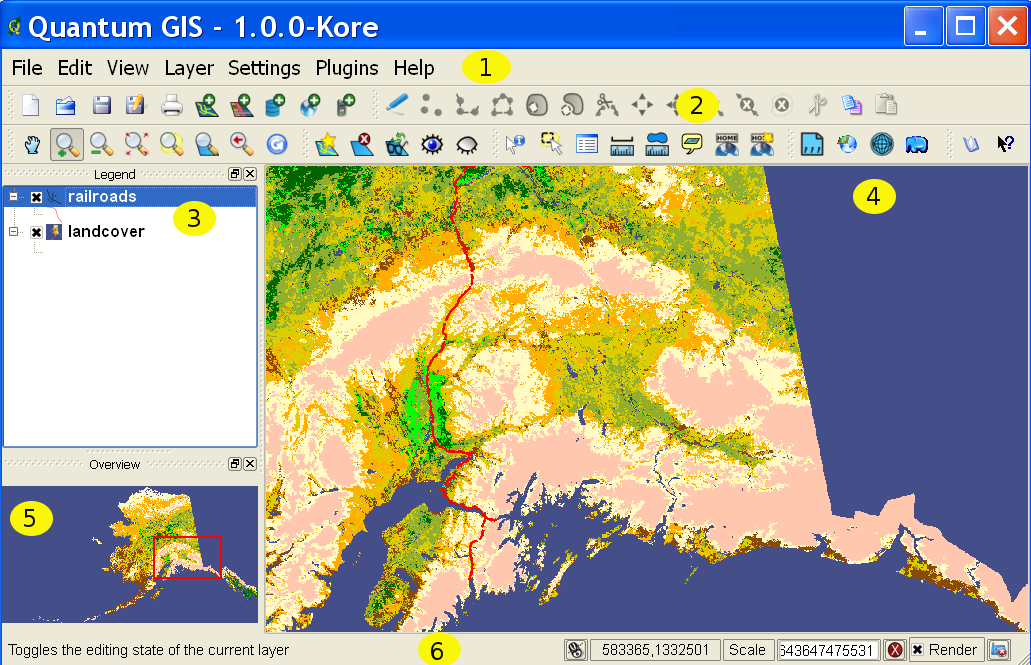
\includegraphics[clip=true, width=17cm]{startup1_0_0}
\end{center} 
\end{figure}


